%\documentclass[letterpaper, onecolumn, 10pt]{article}
%\linespread{2.4}
\documentclass[letterpaper, twocolumn, 10pt]{article}
\usepackage{usenix}
%\linespread{0.99}

\usepackage{multirow}
\usepackage{comment}
\usepackage{epsfig}
%\usepackage{kotex}
%\usepackage{amsmath}
\usepackage{amssymb}
\usepackage{multirow}
\usepackage{url}
\usepackage{subfig}
\usepackage{color}
\usepackage{xcolor}
\usepackage{cases}
\usepackage{graphicx}
%\usepackage{float}
\usepackage{caption}

\renewcommand{\figurename}{Fig.}

\begin{document}

\title{
\vspace{-14pt}
\bf PCStream: Automatic Stream Allocation Using Program Contexts}

%\numberofauthors{1}
\author{
	{\rm Taejin Kim$^1$, Sangwook Shane Hahn$^1$, Sungjin Lee$^2$,} \\ 
	{\rm Jooyoung Hwang$^3$, Jongyoul Lee$^3$, and Jihong Kim$^1$} \\
	\and
	$^1$Seoul National University, $^2$DGIST, $^3$Samsung Electronics
	}


\maketitle
%\thispagestyle{empty}
\pagestyle{empty}
\subsection*{Abstract}
\vspace{-9pt}
We propose a fully automatic stream management technique, called {\sf PCStream}, 
for multi-streamed SSDs.
{\sf PCStream} is based on our observation that data lifetimes can be reliably predicted using
write program contexts.  
By extracting program contexts during runtime,  
{\sf PCStream}  automates the data-to-stream mapping.  
When data mapped to the same
stream show large differences in their lifetimes, {\sf PCStream}
moves the long-lived data of the current stream to 
its substream during garbage collection.
Our experimental results 
show that {\sf PCStream} 
can reduce the garbage collection overhead as much as a highly-optimized 
manual stream management technique 
while no code modification is necessary.

\section{Introduction}
Multi-streamed SSDs provide a special mechanism,
called streams, for a host system to prevent data with different lifetimes 
from being mixed into the same block~\cite{MultiStream}.
Streams, when properly used, can significantly improve both the performance and lifetime of flash-based SSDs by reducing
the garbage collection overhead~\cite{MultiStream, FStream, AutoStream, Level}.  
In order to achieve high performance on multi-streamed SSDs, data with similar 
future update times~\cite{PCHa}
should be allocated to the same stream.
However, since it is difficult to know the future update times {\it a priori} when they are written,
many existing techniques make stream allocation decisions both {\it statically} and {\it manually} by relying on 
programmers' understanding on I/O characteristics of applications/file systems~\cite{MultiStream,FStream}.  
Our long-term goal is to develop a new stream allocation technique, 
which completely automates the task of stream allocation without any direct involvement from programmers.

In order to evaluate the existing stream allocation techniques, 
we view that at least three following  requirements should be satisfied 
by an ideal stream allocator {\sf IdealStream}.   
An ideal stream allocator {\sf IdealStream} needs to
meet at least three requirements.  
First, {\sf IdealStream} should be fully automatic without requiring manual work from
programmers.   
Second, {\sf IdealStream} must allocate streams based on the data lifetime.  
When two data have different lifetimes, they should not be allocated to the same stream.   
Third, {\sf IdealStream} should be able to change the data-to-stream mapping during the run time, 
reflecting varying data lifetimes.
As summarized in Table 1, however, none of existing stream management 
techniques~\cite{MultiStream,FStream,AutoStream} meets three requirements.  
Except for AutoStream~\cite{AutoStream}, 
both FStream~\cite{FStream} and ManualStream~\cite{MultiStream}
\footnote{For a description purpose, we call the technique 
used in~\cite{MultiStream} by ManualStream.}
are manual techniques 
which need to modify 
file system or applications.
Although AutoStream automatically allocates streams at the device driver level, 
its stream allocation policy does not work with modern append-only workloads such as RocksDB or Cassandra.  
Unlike conventional update workloads where data written to the same logical block address (LBA) 
shows a strong update locality, 
the recent append-only workload completely decouples the data lifetimes from LBAs.  
For example, as will be shown in Section 2, in RocksDB, 
a chunk of data written to a fixed 
LBA range have widely varying data lifetimes over times.  

\begin{table}[b]
	\vspace{-15pt}
	\centering
	\caption{Limitations of existing studies}
	\vspace{-5pt}
	\begin{tabular}{c|ccc}\hline
		\renewcommand{\arraystretch}{0.5}
		& lifetime- & \multirow{2}{*} {automatic} & \multirow{2}{*} {adaptable} \\
		 & based     &                           &                           \\ \hline\hline
		\renewcommand{\arraystretch}{0.5}
		Multi- &\multirow{2}{*}  o & \multirow{2}{*} x & \multirow{2}{*} x \\
		Streaming &                &                   &                   \\\hline
		\renewcommand{\arraystretch}{3}
		FStream & o & x & x \\ \hline
		\renewcommand{\arraystretch}{3}
		AutoStream & x & o & o \\ \hline
	\end{tabular}
\end{table}

In this paper, we propose a new stream management technique, called {\sf PCStream}, 
which meets all three requirements.   
The key insight behind {\sf PCStream} is that
data lifetimes should be monitored at a higher abstraction level than the LBA level.   
Since a program context represents a particular execution path of a program, 
when data lifetimes are observed at the same program context, 
they tend to be similar~\cite{PCHa}. 
For example, in the context of managing the RocksDB log file, 
log data are written when key-value pairs are temporarily stored in the memory, 
and log data are deleted if the key-value pairs are flushed to storage~\cite{RocksDB}.
In a typical workload, log data has a similar lifetime because the key-value pairs 
reside in the memory at a similar time.

By identifying program contexts during the run time, 
{\sf PCStream} can directly map a program context to a stream.   
While {\sf PCStream} works efficiently for most workloads, the lifetime of data written from
a single program context can be quite fluctuating, thus making a pure PC-based approach less effective.   
In {\sf PCStream}, we modify stream allocations when such PC is observed. 
The main drawback of the mixed lifetimes is that 
long-lived data remains as a valid page, worsening garbage collection efficiency.
In order to separate the long-lived data from the others,
we assign an additional stream, called substream, to copy valid pages
of the original stream.

Our experimental results show that {\sf PCStream} can reduce the
garbage collection overhead as much as manual stream
management techniques while no code modification is necessary.
For a RocksDB benchmark, {\sf PCStream} improved WAF by 40\% over 
the existing automatic technique.

The rest of this paper is organized as follows. 
We explain the key motivations behind {\sf PCStream} in Section 2. 
Section 3 describes the main modules of the {\sf PCStream} allocator.
The experimental results are shown in Section 4. 
Finally, we conclude in Section 5 with a summary and future works. 

\begin{comment}
...
Recent studies have used two strategies to utilize the stream feature.
One is to classify the application data into different streams based on an understanding
of the expected lifetime of those data~\cite{MultiStream},~\cite{FStream}. 
This manual stream assignment requires the programmer or system manager to 
fully understand the lifetime characteristics of the data, such as different levels
of a log-structured merge tree or the file extension of commitlog file.
Also when multiple applications try to assign streams, a centralized stream assignment
is required to avoid conflicts.
The other is to automate the process of mapping write I/O operations to an SSD stream~\cite{AutoStream}.
However, since AutoStream relies on the past LBA access patterns, 
it is not practical when the data are written in append-only manner, e.g. RocksDB or Cassandra.

Usually, the lifetime of data is determined by its purpose.
For example, files such as the write ahead log in RocksDB are quickly deleted, 
while write-once data is kept at the bottom level of the LSM-tree for a long time.
Our approach is motivated by the observation that the purpose of the application can be defined as
the execution path of function calls that lead to a write system call, called program context.
In this paper, we take the program context information as a lifetime hint for the automatic stream allocation. 
\end{comment}


\vspace{-13pt}
\section{Basic Idea}
\vspace{-5pt}
\subsection{Fallacy: LBA-based lifetime prediction}
%\vspace{-5pt}
Many existing data separation techniques such as~\cite{AutoStream, HotCold} 
estimate the data lifetime based on the update frequency of LBAs.  
For example, AutoStream~\cite{AutoStream} assumes that, if
some LBAs are frequently rewritten by applications, those LBAs hold hot data.
This LBA-based lifetime prediction 
approach, however, does not work well with recent data-intensive 
applications where a majority of
new data are written in an append-only manner.  



In order to illustrate a mismatch between an LBA-based predictor and 
append-only workloads, we analyzed the write pattern of 
RocksDB~\cite{RocksDB}, which is a
popular key-value store based on the LSM-tree algorithm~\cite{LSM}.
Fig.~\ref{fig:lba_lifetime}(a) shows how LBAs may be related 
to data lifetimes\footnote{The lifetime of data is defined to be 
the number of write requests between when the data is first written 
and when the data is invalidated by an overwrite or a TRIM command.}
in RocksDB~\cite{RocksDB}.  
As shown in Fig.~\ref{fig:lba_lifetime}(a), 
there exists no strong correlation between the LBAs and lifetimes in RocksDB.  
This scatter plot is in sharp contrast with one for update workloads 
where a few distinct LBA regions have short lifetimes while others 
have very long lifetimes.

We also analyzed 
if the lifetimes of LBAs change under some predictable patterns over times 
although the overall lifetime distribution shows large variances.
Fig.~\ref{fig:lba_lifetime}(b) shows a scatter plot of data lifetimes over the logical time 
for a specific 1-MB chunk with 256 pages. 
As shown in Fig.~\ref{fig:lba_lifetime}(b), 
for the given chuck, data lifetimes vary in a random fashion
(although some temporal locality is observed).
\begin{comment}
Over the logical time, the lifetime of data written to the chunk 
varies in an unpredictable fashion.  
For example, at the logical time 10, the lifetime was 1 but it increases about 
2.6 million around the logical time 450 
followed by a rapid drop around the logical time 600. 
\end{comment}
Our illustration using RocksDB strongly suggests that under append-only
workloads, LBAs are not useful in deciding data lifetimes.

\vspace{-10pt}
\subsection{Program context as a lifetime predictor}
%\vspace{-5pt}
In developing \textsf{\small PCStream}, our key insight was that in most applications 
(regardless of their I/O workload characteristics), 
a few dominant I/O activities exist for an application
and each dominant I/O activity   
represents the application's important I/O context (e.g., for logging or for flushing). 
Furthermore, most dominant I/O activities tend to have distinct data lifetime patterns.
In order to distinguish data by their lifetimes, therefore, 
it is important to effectively distinguish dominant I/O activities from each other.  
For example, in update workloads, 
LBAs alone were effective in separating dominant I/O activities.  

\begin{figure}[t]
	\centering
	\vspace{-7pt}
	\subfloat[Lifetime patterns over LBAs]{\includegraphics[width=0.25\textwidth]{figure/lba_lifetime2}}  % data from 0/03031641
	\subfloat[Lifetime patterns over time]{\includegraphics[width=0.22\textwidth]{figure/lifetime_in_chunk2}}
	%\includegraphics[width=0.9\linewidth]{figure/lba_lifetime} 
	%\vspace{-10pt}
	\vspace{-7pt}
	\caption{Lifetime distributions over addresses and times.} %shane part
		\label{fig:lba_lifetime}
	\vspace{-17pt}
\end{figure}

\begin{comment}
In developing PCStream, we started from a simple question: 
how can we extract I/O context from an application? 
For example, in RocksDB, logging, flushing and compaction can be regarded
as different I/O contexts.
RocksDB appends write-ahead logs to storage to ensure data
persistence.  Those logs have short lifetimes because they are quickly deleted
after original data are persistently stored.
The flush module (which materializes the content of a memtable in
DRAM, called an L0 table, to an L1 table in the storage) generates data
with relatively short lifetimes. This is because an L1 table will be flushed to
an L2 table and be removed in the near future. Conversely, a compaction module
writes long-lived data that are unlikely to be removed for a long time.

The above observation implies that, if we are able to know the detailed
behaviors of append-only applications, data with different lifetimes can be
isolated in separate streams in an SSD. As mentioned before, a common
solution~\cite{MultiStream} to realizing this is manually modify an application
code so that each module assigns a unique stream ID to data it generates.
However, owing to considerable implementation efforts required to modify
individual applications, this approach is not widely used in practice.
\end{comment}

In this paper, we argue that a program context is an efficient  general-purpose
indicator for separating dominant I/O activities regardless of the type of I/O
workloads.  Since a PC represents an execution path of an application which
invokes write-related system functions such as {\tt write()} and {\tt writev()}
in the Linux kernel,  we represent the PC by summing program counter values of
all the functions along the execution path which leads to a write system call.
In RocksDB, for example, dominant I/O activities include logging, flushing and
compaction.  Since they are invoked through different function-call paths, we
can easily identify dominant I/O activities of RocksDB using PCs.  For example,
Fig.~\ref{fig:getpc}(a) shows an execution path for flushing in RocksDB.  The
sum of program counter values of \texttt{Run()}, \texttt{WriteLevel0Table()},
and \texttt{BuildTable()} is used to represent the PC for the flushing
activity.  Note that using the program context to distinguish data lifetimes is
not new.  For example, Ha {\it et al.} proposed a data separation technique
based on the program context~\cite{PCHa}.   However, their work was neither
designed for append-only workloads nor for modern multi-streamed SSDs.

\begin{figure}[b]
\centering
\vspace{-27pt}
\hfill
	\subfloat[Logging (PC)]{\includegraphics[width=0.21\textwidth]{figure/type_1}} % data from 4/03031953 
	\hspace{2pt}
	\subfloat[Logging (manual)]{\includegraphics[width=0.21\textwidth]{figure/pcID_2}}
\hfill
\vspace{-1pt}
	\subfloat[Flushing (PC)] {\includegraphics[width=0.21\textwidth]{figure/type_3}}
	\hspace{2pt}
	\subfloat[Flushing (manual)]{\includegraphics[width=0.21\textwidth]{figure/pcID_3}}
\vspace{-7pt}
\caption{Data lifetime distributions of different PCs.} 
\label{fig:types_and_PCs}
%\vspace{-15pt}
\end{figure}


In order to validate our hypothesis that PCs can be useful for predicting
lifetimes by distinguishing dominant I/O activities, we conducted experiments
using RocksDB, comparing the accuracy of identifying dominant I/O activities
using two different methods.  First, we manually identified dominant I/O
activities by inspecting the source code. Second, we automatically decided
dominant I/O activities by extracting PCs for write-related system functions.
Fig.~\ref{fig:types_and_PCs} illustrates two dominant I/O activities matched
between two methods.   As shown in Fig.~\ref{fig:types_and_PCs}(a)
and~\ref{fig:types_and_PCs}(b), the logging activity of RocksDB is correctly
identified by two methods.  Furthermore, from the logging-activity PC, we can
clearly observe that data written from the PC are short-lived. Similarly,
from Fig.~\ref{fig:types_and_PCs}(c) and~\ref{fig:types_and_PCs}(d), we observe
that data written from the flushing-activity PC behaves in a different fashion.
For example, data from the flushing-activity PC remain valid a lot longer than
those from the logging-activity PC.



\vspace{-7pt}
\section{Design of \textsf{\normalsize PCStream}}
\vspace{-5pt}
We describe in detail the proposed automatic stream management technique, 
\textsf{\small PCStream}.  We first explain how we automatically extract PCs during
run time and describe how multiple PCs are mapped to streams in an SSD.
In order to mitigate the side effect of a few outlier PCs with large lifetime variances, 
we introduce `substreams' based on a two-phase
stream assignment technique.
%{\it The PC extractor module}, which is implemented in the ... as part ... of a
%system call handler, computes a PC signature (i.e., a sum of program counter
%values) for each write-related system function. 추가 동작 설명..


Fig.~\ref{fig:architecture} shows an overall organization of \textsf{\small PCStream}.
\textit{The PC extractor module}, which is implemented in the Linux kernel as
part of a system call handler, 
computes a PC signature, which is used as a unique ID for each program context.  
We use the signature program counter~\cite{PC} as a PC signature 
by summing program counter values along the execution path to a write-related system function 
(e.g., {\tt write()}).  
With the PC signature, we can monitor the data lifetime of each write at the program context level. 
A PC signature is stored
in an inode data structure of a file system (modified for \textsf{\small PCStream})
and is delivered to \textit{the lifetime analyzer module} which estimates
expected lifetimes of data belonging to a given PC in the block device level.
In order to efficiently detect the end of data lifetime in append-only
workloads, the lifetime analyzer also intercepts TRIM~\cite{TRIM} requests. %from a file system.  %shane part
Based on the lifetime information, \textit{the PC-to-stream
mapper module} clusters PCs with similar lifetimes and maps them together to
the same stream ID.  This mapping is required because 
the number of streams in an SSD is generally less than the number of PCs in host applications.

\vspace{-10pt}
\subsection{Automatic PC computation}
%\vspace{-5pt}
As mentioned earlier, a PC is represented by a PC signature which is defined as
the sum of program counter values along the execution path of a function call that
finally reaches a write-related system function. A function call involves
pushing the next program counter, which is used as a return address, to the
stack followed by pushing a frame pointer value.  In general, by using frame
pointer values, we are able to back-track the stack frames of the process and
selectively get return addresses for generating a PC signature.  For example,
Fig.~\ref{fig:getpc}(a) shows the abstracted execution path for flushing data
in RocksDB and Fig.~\ref{fig:getpc}(b) illustrates how a PC signature is obtained
by back-tracking the stack.  
Since a frame pointer value in the stack holds the address of the previous
frame pointer, the PC extractor can easily obtain return addresses and
accumulate them to compute a PC signature. (The return addresses are pushed
before calling the \textsf{\small  write()}, \textsf{\small  BuildTable()} and \textsf{\small 
WriteLevel0Table()} functions.)

\begin{figure}[t]
	\centering
	\vspace{-7pt}
	\includegraphics[width=0.6\linewidth]{figure/architecture4}
	\vspace{-10pt}
	\caption{An overall architecture of \textsf{\small PCStream}.}
	\label{fig:architecture}
	\vspace{-15pt}
\end{figure}

%The PC extractor obtains and accumulates each
%return address, which is pushed before calling the \textsf{\small  write()}, \textsf{\small 
%BuildTable()} and \textsf{\small  WriteLevel0Table()} functions, by referring the frame
%pointer which holds the address of the previous frame pointer.

%Unfortunately, C/C++ compilers often optimize an output code so
%that it does not use a frame register if possible.  
The frame pointer-based approach for computing PC signatures, however, is not
always possible because modern C/C++ compilers often do not use the frame
pointer for improving the efficiency of register allocation.
One example is a
{\tt -fomit-frame-pointer} option of GCC~\cite{GCC}. 
%While it is effective in saving
%precious resources like CPU registers, this makes it difficult for us to
%back-track return addresses only. 
Although this option allows the frame pointer to be used as a general-purpose
register for high performance, it makes very difficult for us to back-track
return addresses along the call chains.  

\begin{figure}[b]
%	\vspace{-10pt}
	\centering
	\vspace{-16pt}
	\subfloat[An abstracted execution path for flushing data.]{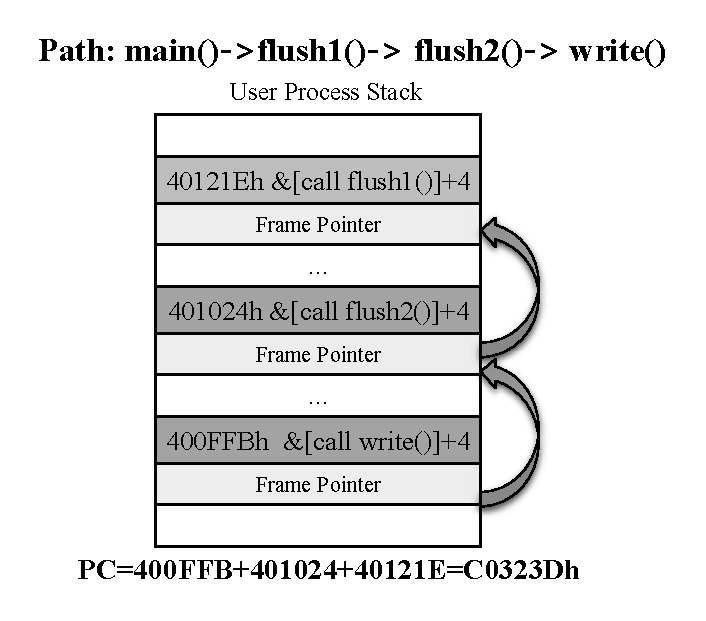
\includegraphics[width=0.45\textwidth]{figure/getpc_1}}  
	\vspace{-10pt}
	\hfill
	\subfloat[with the frame pointer.]{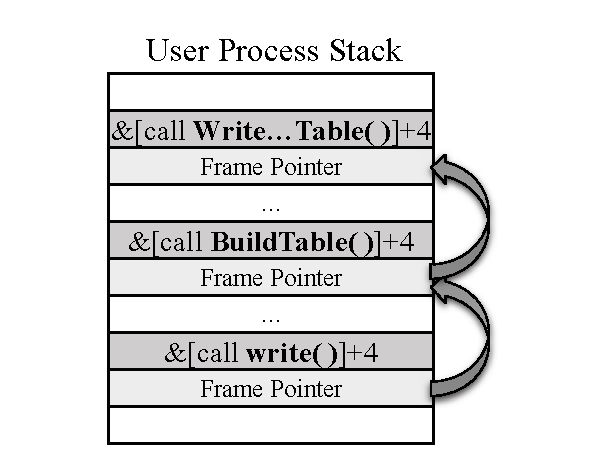
\includegraphics[width=0.245\textwidth]{figure/getpc_2}}
	\subfloat[without the frame pointer.]{\includegraphics[width=0.25\textwidth]{figure/getpc_3}}
	\vspace{-10pt}
	%\caption{An example execution path and its PC extraction methods.}
	\caption{An example execution path and its PC extraction.} %shane part
	\label{fig:getpc}
\end{figure}

In \textsf{\small PCStream}, we employ a simple but effective workaround 
for backtracking the call stack when the frame pointer is not used.
When a write system call is made, we scan the every word in the stack and check
if it belongs to the process's code segment.  If the scanned stack word holds a
value within the address range of the code segment, we assume that it is a
return address.  Since scanning the full stack takes too long, we stop the
stack scanning procedure when a sufficient number of return address candidates
are found.  In the current version, we stop when 5 return address candidates
are found.  Although quite ad-hoc, a restricted scan is effective in
distinguishing different PCs because two different PCs
follow the same execution path up to five caller functions.   
cannot follow the same execution path to write system functions.  
(If they do, they are the same PC.) In our evaluation
with a 3.4 GHz CPU machine, the performance overhead of the restricted scan was
almost negligible, taking only 300-400 $n$sec per write system call.



\vspace{-10pt}
\subsection{PC lifetime prediction}
The prediction of PC lifetimes is rather complicated. 
The data lifetime of the append-only workload is defined 
from when a write request is issued until the TRIM command~\cite{TRIM} is issued to 
the corresponding address.
Before issuing a write request, the lifetime analyzer
maintains the written time and the address as well as the PC signature.
Upon receiving TRIM
commands destined for those LBAs, the lifetime analyzer is able to measure the
exact lifetime of those data. 
Note that, the
same PC may generate multiple data streams with different lifetimes.
We take the average lifetime as the PC's lifetime.

\vspace{-10pt}
\subsection{Mapping PCs to SSD streams}
\vspace{-5pt}
The last step in \textsf{\small PCStream} is to map
a group of PCs with similar lifetimes to an SSD stream.
This is because each SSD supports a limited number of stream IDs. For
example, SSDs used in \textsf{\small FStream}~\cite{FStream} and \textsf{\small AutoStream}~\cite{AutoStream}
support only 9 and 16 streams, respectively. To properly group multiple PCs,
the PC-to-stream mapper employs a simple 1-D clustering algorithm.  For all the
PCs, the mapper internally builds a 1-D array sorted by PCs' lifetimes.  Given
an available SSD stream number, it runs the clustering algorithm and determines
the best arrangement of PCs into different classes.  For adapting to changing
workloads, reclustering operations should be regularly performed. Since the
number of PCs created by applications is not limited, the clustering algorithm
must be efficient enough to quickly handle many PCs. Our goal in this work is
to confirm the feasibility of using PCs, so we leave
those issues as our future work.

\vspace{-10pt}
\subsection{Two-phase stream assignment}
\vspace{-5pt}

For most PCs, their lifetime distributions tend to have small variances.  
However, we observed that a few outlier PCs which have large lifetime variations. 
For example, when multiple I/O contexts are covered by the same write system function, 
the corresponding PC may represent several I/O contexts whose data lifetimes are quite different.   
Such a case occurs, for example, in the compaction module of RocksDB.
RocksDB maintains
several levels, L1, ..., L$n$, in the persistent storage, except for L0 (or a
memtable) stored in DRAM.  Once one level, say L2, becomes full, all the data
in L2 is compacted to a lower level, i.e., L3.  It involves moving data from L2
to L3, along with the deletion of the old data in L2.  In the
LSM tree~\cite{LSM}, a higher level is smaller than a lower level 
(i.e., the size of (L2) $<$ the size of (L3)). 
Thus, data stored in a higher level is invalidated more frequently than those kept
in lower levels, thereby having shorter lifetimes.

%Once the L1 becomes full,
%\textit{all} the data kept in the L1 are moved to the L2 by the compaction
%module.  The same operation is applied to the other levels (i.e., L3, ...,
%L$n-1$).  The compaction involves reading and writing data from a higher level
%(e.g., L1) to a lower level (e.g., L2).  The data in a higher level (e.g., L1)
%is then removed.  

%While the program context can be used as a useful indicator that determines the
%lifetime of data, we also observe that the same PC could generate data 
%with diverged lifetimes. One of the representative examples is the compaction
%module of RocksDB. RocksDB maintains several levels, L1, ..., L$n$, in the
%persistent storage, except for L0 (or a memtable) stored in DRAM.  Data flushed
%from the memtable are first written to the L1.  Once the L1 becomes full,
%\textit{all} the data kept in the L1 are moved to the L2 by the compaction
%module.  The same operation is applied to the other levels (i.e., L3, ...,
%L$n-1$).  The compaction involves reading and writing data from a higher level
%(e.g., L1) to a lower level (e.g., L2).  The data in a higher level (e.g., L1)
%is then removed.  In the LSM-tree, a higher level is smaller than a lower
%level. Thus, data stored in a higher level is invalidated sooner than data kept
%in lower levels, thereby having much shorter lifetimes.

Unfortunately, in the current RocksDB implementation, the compaction step is supported 
by the same execution path (i.e., the same PC) regardless of the level.
Therefore, the PC for the compaction activity cannot effectively separate data with 
short lifetimes from one with long lifetimes.
Fig.~\ref{fig:compaction}(a) shows 
the lifetime distribution collected from the compaction-activity PC.  
Since this distribution includes lifetimes of data written from all the levels, 
its variance is large.  
When we manually separate the single compaction step into several per-level compaction steps, 
as shown in Figs. 5(b) and 5(c), the lifetime distributions of per-level compaction steps 
show smaller variances.   
In particular, L2 and L3 show distinct lifetime distributions from L4.
Data from L1 are likely to have shorter lifetime, while L4 has generally
long-lived data.

\begin{figure}[!t]
\centering
\vspace{-7pt}
\hspace{2pt}
\subfloat[compaction: all levels]{\includegraphics[width=0.23\textwidth]{figure/pc_3b}}
\subfloat[compaction: L2]{\includegraphics[width=0.23\textwidth]{figure/type_4b}}  % data from 4/03040047
\hfill
\vspace{-10pt}
\subfloat[compaction: L3]{\includegraphics[width=0.23\textwidth]{figure/type_5b}}
\subfloat[compaction: L4] {\includegraphics[width=0.23\textwidth]{figure/type_6b}}
\vspace{-5pt}
%\caption{The lifetime distribution of the compaction activity.} 
\caption{Lifetime distributions of the compaction activity at different levels.} %shane part
\label{fig:compaction}
\vspace{-15pt}
\end{figure}

In order to automatically assign data from the same PC to different SSD streams
according to their lifetimes, we devised a two-phase method that decides SSD
stream IDs both in a host level and in an SSD level.
For such a PC (e.g. the compaction-activity PC {\it pID}), \textsf{\small PCStream} assigns a
stream {\it sID} at the host level.
To separate long-lived data of 
{\it pID} (e.g., L4 data) from short-lived (future) data of {\it pID} (e.g., L1 data), 
we move the long-lived data of {\it sID} to its substream during garbage collection.   
Conceptually, a substream is used to re-separate data in the same stream so that 
future short-lived data cannot be mixed with past long-lived data in the same block.


\section{Experimental Results}
For our evaluation, we implemented PC extractor module at the 
system call layer 
and PC-Lifetime analyzer and PC-to-Stream mapper module 
at the block device layer in the Linux kernel version 4.5.

In order to evaluate the effectiveness of {\sf PCStream},
we implemented the multi-stream feature and substream concept
to the in-house SSD emulator
based on the open flash development platform~\cite{AMF}.
The number of streams was set to 8 for the evaluation.
The SSD emulator was 8 GB with four channels with four ways, and 
the number of blocks per a parallel unit was 512 and
the number of pages per block was 256 with 4KB-sized page.
Due to the limited capacity of the emulator, 
we scaled down RocksDB configuration.
The base file size is set to 8 MB
with the size of key-value is 8 KB and the number of levels was set to 4.
However, the size of level multiplier is remained to be 10 as an usual setting,
which means the size of the next level is 10 times larger than previous level,
to maintain the level access patterns during the compaction.

For benchmarks, we used three scenarios of db\_bench of RocksDB.
The update random scenario (read-modify-write for random keys), {\tt UR}, and 
the append random scenario (read-modify-write with growing values), {\tt AR}, are
for intensively updating key-value pairs.
For each scenario, about 900000 keys are inserted.
The fill random scenario (write values in random key order), {\tt FR}, 
inserts 300000 key-value pairs 
after 70\% of the device capacity was filled.

For the comparison, 
we also implemented Autostream, manual technique, and
baseline which does not use the stream allocation policy.
We compared WAF of the existing techniques with {\sf PCStream}
for each scenario.

\begin{figure}[t]
	\centering
	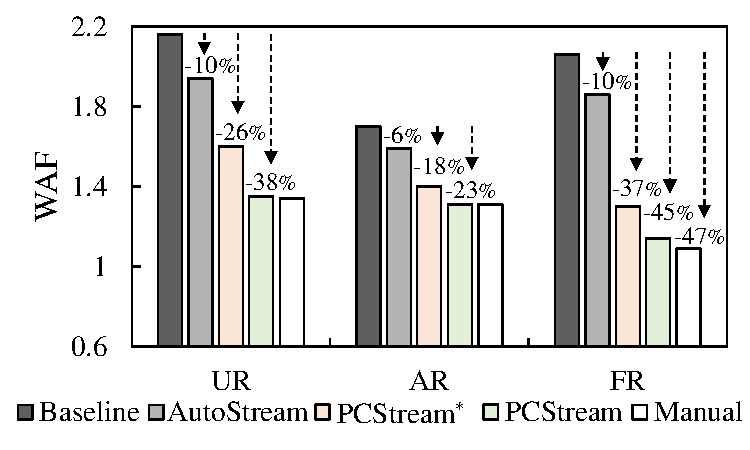
\includegraphics[width=0.8\linewidth]{figure/result_emul}
	\vspace{-10pt}
	\caption{The WAF comparison on the emulator.}
	\label{fig:result_emul}
	\vspace{-15pt}
\end{figure}

As shown in Fig.~\ref{fig:result_emul}, 
{\sf PCStream} reduces WAF by up to 45\% over the baseline technique. 

In order to evaluate the effectiveness of {\sf PCStream},
we used Samsung PM963 480GB SSD (with 8 streams).
As a warming workload, we wrote a single file sequentially to fill 90\%
of logical device capacity, to ensure that 90\% of logical space stays valid
throughout the test.

\begin{figure}[t]
	\centering
	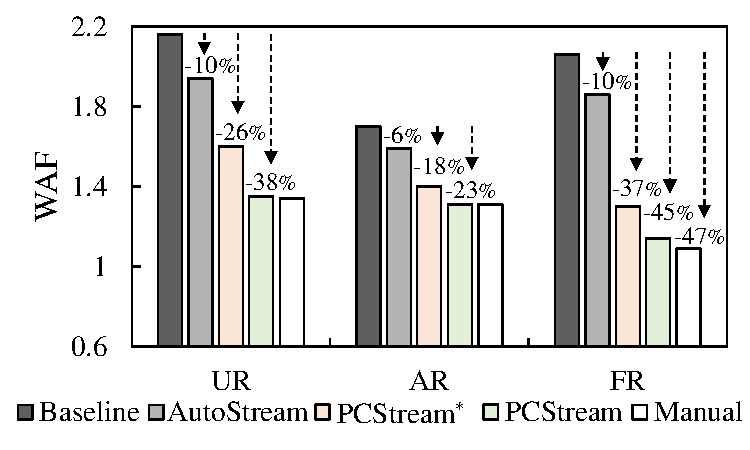
\includegraphics[width=0.8\linewidth]{figure/result_emul}
	\vspace{-10pt}
	\caption{The WAF comparison on the SSD.(temporarily placed to check paper length)}
	\label{fig:result_SSD}
	\vspace{-15pt}
\end{figure}



\section{Conclusion}
In this paper, we presented a new fully automatic stream management technique,
called PCStream, which can improve the accuracy of data separation
using the application level information.
In the modern append-only workload, since the hotness of data is regardless of 
the its address, 
LBA-based existing automatic stream management technique have limitations on 
identifying the hotness of data.
PCStream was motivated by our observation that data lifetimes can be
reliably predicted using write program contexts which is from the higher
abstraction level than LBAs.
By allocating the identified PCs into streams according to the mapping policy,
PCStream can separate different lifetime data. 
For some PCs showing various lifetime, PCStream moves the long-lived data of 
current stream to its substream during the garbage collection.
Experimental result showed that PCStream reduces WAF by 40\% over the existing
automatic technique.
Future work ...


\vspace{-14pt}
\section*{Acknowledgments}
\vspace{-7pt}

This work was supported by the National Research Foundation of Korea (NRF) 
grant funded by the Korea government (Ministry
of Science and ICT) 
(NRF-2015M3C4A7065645 and NRF-2018R1A2B6006878).
The ICT at Seoul National University
provided research facilities for this study. 
Sungjin Lee was supported by
the NRF grant funded by the Korea government 
(Ministry of Science and ICT) 
(NRF-2017R1E1A1A01077410) and 
the DGIST R\&D Program of the Ministry of 
Science and ICT (18-EE-01).
(Corresponding Author: Jihong Kim)
\bibliographystyle{abbrv}
\bibliography{sigproc}
\begin{thebibliography}{00}

%\bibitem{mohan}
%V. Mohan, T. Siddiqua, S. Gurumurthi, and M. Stan, 
%``How I Learned to Stop Worrying and Love Flash Endurance,'' 
%in \textit{Proceedings of the Workshop on Hot Topics in Storage and File Systems}, 2010.

\end{thebibliography}



\end{document}
